% !TEX root = ../thesis-example.tex
%
\chapter{Interface sensible / hardware}
\label{ch:interfaces}

\cleanchapterquote{Komponieren heißt: über die Mittel nachdenken.\\
Komponieren heißt: ein Instrument bauen.\\
Komponieren heißt: nicht sich gehen, sondern sich kommen lassen.\\
.}{Helmut Lachenmann}{1986}

\cleanchapterquote{Fingers are not to be despised: they are great inspirers, and, in contact with a musical instrument, often give birth to subconscious ideas which might otherwise never come to life.}{Igor Stravinsky}{1936}

\vspace{-1em}
\begin{itemize}[noitemsep]
\item Faire évoluer une interface en la raffinant (De Laubier, VG).
\item Faire évoluer une interface en rajoutant des choses (Patricia Dallio)
\item Faire évoluer en supprimant des choses (Dumaux)
\item Partir de l'objet (Patrick Saint Denis)
\end{itemize}

%--------------------------------------------------------------
\section{Interface gestuelle ou interface sensible?}

\noindent Il est souvent question ``d'interface gestuelle'' lorsqu'on pense aux \glspl{IHM} utilisées pour l'interaction musicale. Comme nous l'avons vu au chapitre précédant, le geste occupe une part importante de l'interaction musicale mais les interfaces de jeu ne se restreignent pas nécessairement à la captation du geste : elle peuvent être sensible à la température, la lumière\footnote{Voir par exemple les œuvres \textit{Light Thing} de Leaf Cutter John (\url{https://youtu.be/2jIlLHfSEfs}), ou encore \textit{Light Music} de Thierry de Mey}, à la couleur, et réagir de manière générale à différentes conditions environnementales.\\
\indent Par ailleurs, le geste possède un certain nombre de qualités qui ne sont pas forcément captées par l'interface, alors qu'elle sont effectivement vues et ressenties par le musicien et par le public, et contribuent ainsi à la performance, comme nous l'avons présenté au chapitre précédent.\\
\indent Enfin, le "geste" qui vient contrôler les processus sonores dans les \glspl{DMI} peut être de nature virtuelle, prendre la forme de motifs pré-enregistrés qui peuvent être issus de toute sorte de source de données interprétées en tant que flux temporels, tels que peut-être le cas dans la sonification de données ou l'utilisation de modèles intermédiaire. Cet aspect là sera décrit plus en détail dans le chapitre \ref{ch:algorithms}.\\
\indent Il semble ainsi préférable de parler d'\textit{interface sensible}, plutôt que d'\textit{interface gestuelle} pour décrire les dispositifs d'interaction numériques pour la musique, leur caractéristique commune étant l'usage de capteurs (\textit{sensors}).


%%%%%%%%%%%%%%%%%%%%%%%%%%%%%%%%%%%%%%%%%
\section{Composer, interpréter, improviser en live}

\noindent Les \glspl{DMI} intègrent généralement des matériaux pré-composés, que le musicien peut lancer et qui pourront tourner ``tout seul'' (paysages sonores, processus génératifs, drônes, etc.) et une part créée plus directement, qu'elle soit synthèse ou transformation de matériaux.\\
\indent Les différents accès de l'interface de jeu doivent ainsi permettrent d'articuler au mieux ces deux pôles et permettre la gestion du temps à différentes échelles. En particulier, les interfaces multitouch, si elles permettent de gérer aisément de multiples processus lents (qu'on pourra visualiser et ajuster à l'écran), ne permettent guère une réactivité ``percussive'', telle que le permet un pad \gls{MIDI} ou mieux encore, le microphone.\\
\indent La ``granularité'' du contrôle joue également un rôle important dans cette perspective. Entre une note \gls{MIDI} qui ne déclenche qu'un événement ponctuel, un contrôleur continu qui envoie des données chaque fois qu'il est modifié et un capteur échantilloné qui envoie des informations en continu, les possibilités de contrôle seront différentes en terme de réactivité et de finesse de modulation. Il faut donc prévoir les capteurs adéquats pour les processus que l'on souhaite contrôler en aval. Comme le faisait remarquer Max Mathews, cité par Joel Chadabe dans \cite{chadabe_electric_1996}:
\begin{quotation}
	Il faut penser aux systèmes dans leur globalité pour obtenir une quelque chose d'utilisable musicalement - on ne peut pas vraiment développer un capteur sans le mettre en perspective des programmes avec lesquels on va l'utiliser. \footnote{``One has to think of overall systems to get a musically useful thing — you can't really develop a sensor without relating it to the programs that you're going to use it with.'', p. 230}
\end{quotation}
\noindent Ceci n'est pas sans poser problème dans la perspective de modularité d'un \gls{DMI} que l'on aimerait pouvoir faire évoluer et adapter à différents contextes. Un compromis consiste à disposer d'une palette de capteurs différents et de les agencer selon une ergonomie adaptée aux gestes qu'ils invitent, et d'adapter le logiciel, plus souple, à cette configuration.

\section{La part acoustique de l'interface des DMIs}
\label{sec:interfaces:part_acoustique}

\noindent Il faut ici rappeler que les \glspl{DMI}, s'ils se caractérisent par l'usage de la computation numérique, sont aussi nécessairement des instruments électroniques, électriques et acoustiques. Il portent l'héritage de ces différentes technologies et les contraintes propres à ces médias. Mais le phénomène acoustique, omnidirectionnel et tri-dimensionnel dans un système acoustique, est réduit dans l'électronique numérique à un signal mono-dimensionnel\footnote{Nicolas Collins, dressant une liste de traits distinctifs entre hardware et software dans \cite{collins_semiconducting_2013} notait: ``Traditional acoustic instruments are three-dimensional objects, radiating sound in every direction, filling the volume of architectural space like syrup spreading over a waffle. Electronic circuits are much flatter, essentially two-dimensional. Software is inherently linear, every program a one-dimensional string of code.''} et mono-directionnel, introduisant une distinction entre ce qui est ``entrée'' d'une part et ``sortie'' d'autre part. La dimension acoustique des \glspl{DMI} s'intègre donc dans un circuit ouvert ou fermé avec le système de computation via des transducteurs acoustiques, qu'ils soient microphones, en entrée, ou haut-parleurs, en sortie.\\
\indent Paradoxalement, si le résultat acoustique d'un instrument est \textit{in fine} ce qui nous intéresse le plus, la part acoustique de l'instrument numérique est aussi sa part maudite. Les phénomènes de résonnance et qui se produisent naturellement dans l'instrument acoustique, et sont également exploités dans les instruments électriques analogiques (e.g. le feedback entre une guitare électrique et un amplificateur), posent un certain nombre de problèmes lorsqu'on introduit un élément de computation numérique dans un tel système\footnote{Une des raisons à ce problème est l'instabilité consubstantielle aux systèmes bouclés discrets et non-linéaires, mais également, de manière plus générale, la transition entre le domaine réel de l'acoustique et le domaine symbolique de l'informatique implique une analyse du son qui nécessite une modélisation des phénomènes perceptifs, tels que la hauteur, le rythme, etc. utilisés pour le contrôle}.\\
\extra{nombreux synthétiseurs analogiques ont été mis sur le marché, qui articulent cette part d'électronique analogique (pour les filtres et la synthèse) et numérique (pour le  contrôle), afin de pouvoir bénéficier des avantages des deux domaines.}

\subsection{la captation : microphones et transducteurs piezo}

\noindent La possibilité de pouvoir directement entrer du son acoustique dans un système électroacoustique est une pratique très courante chez les musiciens électroacoustiques, et permet des séquences de jeu en prise directe avec des objets concrets dont on pourra transformer le son. En particulier, l'usage de microphones, notamment de transducteur piezo dites ``microphone de contact'', vient redonner une composante acoustique au corps même de l'agencement instrumental. L'intérêt principal réside dans la richesse du signal capté, comme le note Miller Puckette dans \cite{puckette_infuriating_2011}: \iquote{(...) il y a peu chance que le frottement de balais sur un pad de batterie produise quoi que ce soit d'intéressant, alors que faire la même chose sur un instrument qui fonctionne directement avec le signal audio du microphone de contact (comme nous le faisons ici) offre la possibilité de créer une large gamme de sons musicaux utiles\footnote{``(...) sliding a brush over a drum trigger isn’t likely to produce  anything  useful,  whereas  doing  the  same  thingon an instrument that operates directly on the audio signal from the contact microphone (as we do here) has the possibility to create a wide range of useful musical sounds.''}.} L'usage d'algorithmes d'analyse en temps-réel permet, au delà d'effets déjà existants dans le domaine électroacoustique, d'utiliser les caractéristiques du son comme paramètre de contrôle. Une telle approche a été utilisé notamment dans \cite{schwarz_rich_2014} et l'interface Mogees\footnote{\url{https://www.mogees.co.uk}, voir également l'Annexe \ref{appendix:zamborlin}} est principalement basée sur ce principe. 



\subsubsection{Utilisation des piezo dans les différentes DMIs réalisés}
\todo{déplacer cette section dans 4.5?}
\indent \textbf{Sur le Filigramophone}, des cellules piezo sont placées entre une vitre en plexiglass et le chassis contenant la tablette graphique (cf. Figure todo). Cela permet des gestes percussifs, de frottements ou l'utilisation d'objet mis en mouvement (toupies, dés, diques) directement sur la surface, tout en conservant —à travers le plexiglass— l'usage de la tablette qui renvoit les coordonnées horizontale et verticale ainsi que la pression du stylet. Ces transducteurs piezo permettent de capter les différents timbres de la surface plexi, qui présente une certaine élasticité (par rapport au verre) en étant sertie uniquement sur ses bords, et dont la hauteur spectrale est plus grave au centre et plus aigüe sur les bords. Il est également possible de frapper sur le chassis, ce qui permet d'obtenir une autre nuance de timbre (cf. Figure \ref{fig:interface:filigramophone-piezo}).\\
%------------ Figure : filigramophone et xypre piezo -----------
\begin{figure}[!htbp]
	\captionsetup{format=plain}%
	\centering
	\begin{minipage}[t]{0.48\textwidth}
		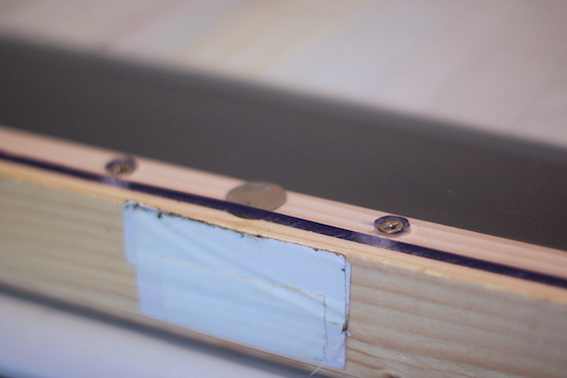
\includegraphics[width=\linewidth]{gfx/05_interfaces/filigramophone-piezo_72dpi.jpg}
		\caption{Transducteur piezo entre la vitre et le chassis sur le Filigramophone}
		\label{fig:interface:filigramophone-piezo}
	\end{minipage}
	\hspace{.02\linewidth}
	\begin{minipage}[t]{0.48\textwidth}
	    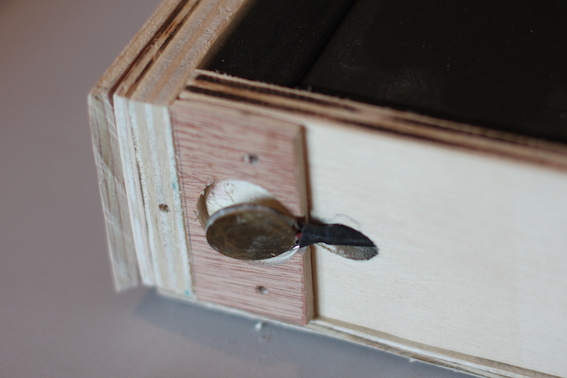
\includegraphics[width=\linewidth]{gfx/05_interfaces/xypre-piezo_72dpi.jpg}
		\caption{Transducteur piezo pseudo-symétrique dans le côté du chassis sur le Xypre v2 (plaque extérieur démontée)}
		\label{fig:interface:xypre_v2-piezo}
	\end{minipage}
\end{figure}
%------------ Figure : filigramophone et xypre piezo -----------
\indent \textbf{Sur le Xypre v1}, la technologie infra-rouge du cadre de détection du multitouch permet d'insérer une vitre plexiglass pour un fonctionnement similaire à celui développé sur le Filigramophone. L'inconvienient qui en résulte est la transmission des vibrations au cadre de détection multitouch et les bruits de plastique qui en résultent.\\
\indent \textbf{Sur le Xypre v2}, l'écran multitouch ne permet pas l'ajout d'un plexiglass les cellules piezo ont été placées sur le côté du chassis, pré-contraints entre le chassis et une plaque de bois plus fine servant de surface de percussion, permettant là-encore de récupérer différentes nuances de hauteur spectrale, utilisée pour la synthèse en aval (cf. figure \ref{fig:interface:xypre_v2-piezo}). La pré-contrainte du piezo est en partie dûe à l'orientation verticale du piezo (qui chuterait, autrement) mais permet également d'utiliser une technique de pseudo-symétrisation du signal du piezo (cf. schéma fonctionnel figure \ref{fig:interface:balancedPiezo} et aperçu figure \ref{fig:interface:xypre_v2-piezo}), qui s'avère très utile quand les transducteurs piezo sont utilisés à proximité d'un écran, source de perturbations électromagnétiques. Romain Michon a étudié les différentes possibilités d'ajouter la possibilité de gestes percussifs sur une tablette multitouch dans \cite{michon_nuance_2016}, ainsi que proposé une solution hybride par l'ajout de capteurs \gls{FSR} placés sous un iPad, modulés en amplitude et récupéré via l'entrée audio d'un iPad. L'intérêt de cette solution est de permettre le calcul de la vélocité des gestes percussifs, en plus de l'aftertouch, mais la combinaison des informations de pression et de coordonnées X/Y, bien que judicieusement contournée par une triangulation des différents \gls{FSR}, reste problématique. Par ailleurs, cette solution utilisant des capteurs de pression, sous la surface rigide de l'iPad ne permet pas d'exploiter la variation de hauteur spectrale en fonction du lieu de frappe, la surface de l'iPad étant trop rigide et les \gls{FSR} inadaptés à cette gamme de fréquences. C'est cette dernière raison qui a motivé la conception du Xypre v2 avec une séparation entre la surface percussive des piezo et la surface de contrôle sur l'écran multitouch.

%-------------------------- Figure : balanced piezo ----------------------------------
\begin{figure}[!htbp]
	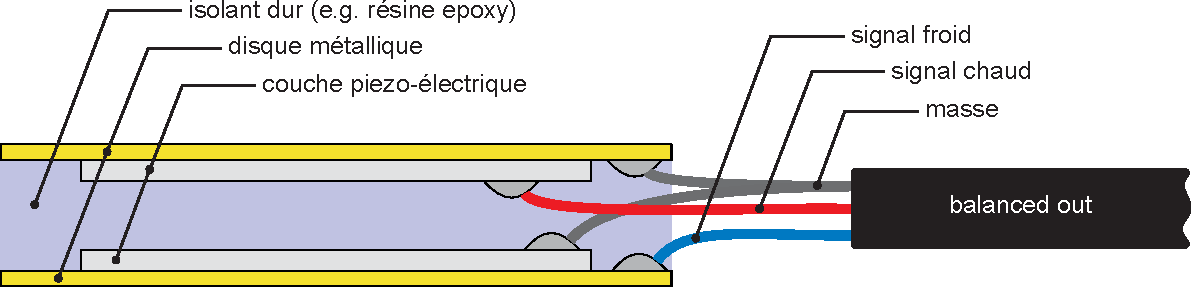
\includegraphics[width=\textwidth]{gfx/05_interfaces/balancedPiezo.pdf}
	\caption{Montage pseudo-symétrique de transducteurs piezo-électriques}
	\label{fig:interface:balancedPiezo}
\end{figure}
%-------------------------- Figure : balanced piezo ----------------------------------

\subsection{la diffusion : haut-parleur et transducteur tactile}

\noindent Dans le cas le plus trivial, l'acoustique des \glspl{DMI} se limite à la membrane du haut-parleur qui transforme \textit{in fine} le signal audio-numérique en son acoustique\footnote{Le choix des haut-parleurs peut jouer un rôle primordial, comme c'est le cas dans la musique acousmatique diffusée sur orchestre de haut-parleur ou ``acousmonium''. Voir en particulier \cite{mooney_sound_2006}}. A la différence des instruments acoustiques, la diffusion et la projection du son est souvent séparée de l'interface gestuelle et, bien souvent, distante du musicien quand elle est ``spatialisée''. La spatialisation du son a en effet joué un rôle essentiel dans la motivation de faire des concert en direct, à une époque où l'arrivée du \gls{CD} et de l'écoute de salon ``haute-définition'', comme le raconte Serge de Laubier en parlant des origines du PSO\footnote{``Processeur Spatial Octophonique'', système de spatialisation inventé par De Laubier en 1986.} et du Méta-Instrument (cf. annexe \ref{appendix:delaubier}) dans les années 1980 : \iquote{Si on entend mieux chez soi, c'est pas la peine de faire des concerts, donc il faut qu'au concert, il y ait une expérience unique qui vaille le coup de se déplacer, d'où réfléchir à un système de spatialisation.}\\
\indent L'essor progressif des transducteurs tactiles à large bande audio depuis la dernière décennie a cependant entrainé l'intégration des haut-parleurs dans le corps de l'instrument, en particulier dans les instruments augmentés tels que la Smart Guitar de HyVibe\footnote{\url{https://www.hyvibe.audio}}. Ce retour acoustique présente plusieurs intérêts :

\vspace{-1em}
\begin{itemize}[noitemsep]
	\item \textbf{offrir au musicien un retour vibratoire }(et/ou auditif), qui lui permet de mieux sentir le résultat sonore et pouvoir plus facilement identifier sa propre production sonore dans le cas de musique d'ensemble;
	\item \textbf{faciliter l'identification et la localisation} auditive de la source sonore et accroître la cohésion entre geste et son et pour le public;
	\item \textbf{bénéficier des propriétés acoustiques des matériaux} structurel de l'instrument, notamment leur rayonnement, beaucoup plus singulier que celui des haut-parleurs (dont la conception est généralement orientée vers un rayonnement et une bande-passante homogène, ``neutre'');
	\item \textbf{introduire du feedback} dans le corps de l'instrument en recaptant cette vibration. Traité avec une latence suffisamment faible, cette possibilité laisse la possibilité de transformer dynamiquement les propriétés acoustiques des matériaux, comme le fait le système HyVibe;
	\item \textbf{communiquer des informations} à l'instrumentiste via un retour vibratoire (cf. TODO mettre un lien vers le développement du frettage virtuel)
\end{itemize}

Sur le Filigramophone, un haut-parleur tactile a été fixé sur la vitre de plexiglass et utilisé à la fois pour le retour vibratoire et la communication d'information, en particulier par frettage virtuel de la surface (cf. section TODO:ref). Le retour vibratoire de l'instrument se distingue toutefois de l'envoi pur et simple du signal audio, la perception tactile ne lui étant pas directement liée. Au lieu de cela, un signal sinusoidal à 70Hz, correspondant à une fréquence de résonnance de la vitre de plexiglass, modulé par l'enveloppe du son final, ainsi que par sa dérivée spectrale, afin de mieux sentir dans les doigts les transitions et les ruptures du son (cf. figure TODO : schéma de principe du patch / développement dans une autre partie ?).

%%%%%%%%%%%%%%%%%%%%%%%%%%%%%%%%%%%%%%%%%
\section{Qualité ergodynamiques}


\subsection{Proprioception}
La proprioception désigne la perception de la position des différentes parties du corps dans l'espace, recouvrant le sens du mouvement (\textit{kinesthésie}) et le sens de la posture (\textit{statesthésie}).


%------------------------------------------------------------
\subsection{Ergodynamisme}
cf. définition de Thor Magnusson
agencement de l’interface, représentation visuelle, repères tactile, frettage

\subsubsection{Le poids du hardware}

\noindent Le hardware, comme son nom l'indique, est solide, matériel, ``dur''. Sa matérialité, son poids affecte sa transportabilité et constitue un facteur contraignant pour le musicien. Sa dématérialisation dans des alternative logicielles —\textit{soft}, plus douces et légères— permet ou non d'intégrer dans les limites acceptables pour leur transport des fonctionnalités offertes par les équipements \textit{hard}.
En particulier, la virtualisation des outils traditionnellement utilisés par les ingénieurs du son (table de mixage, équaliseurs, compresseurs et autres effets) permet leur intégration dans l'instrument lui-même.

(Cf. interview Mamou-Mani.)
Ainsi, Serge de Laubier qui utilisait une table de mixage Yamaha O2R (31kg) motorisée et contrôlée directement depuis son Méta-Instrument, ainsi qu'un échantilloneur EMU (4,5kg) a progressivement conçu des émulation logicielles de ces équipements pour alléger le transport. Par ailleurs, les émulations logicielles permettent de réaliser d'autres fonctions qui n'étaient pas présentes dans les modèles originaux.


\subsubsection{Choix des capteurs et latence}




\subsubsection{Topologie spatiale}

La topologie des capteurs dans l'espace:
\vspace{-1em}
\begin{itemize}[noitemsep]
	\item topologie corpo-centrée (e.g. exosquelette du MI3)
	\item topologie objet, qu'on peut prendre, secouer, etc. (e.g. ``The Sponge'' de Martin Marier)
	\item topologie ``sur table'' objet qu'on ne peut pas déplacer mais autour duquel on peut tourner (e.g. claviers, pad, machine intona rumori de Bernier/Messier ...)
	\item topologie immersive : installation, vidéo, danse (e.g.) (e.g. ``Machine variation'' de Bernier/Messier)
\end{itemize}



\subsubsection{Intégration de l'instrument}

Est-ce que l'instrument est plug'n'play ou va-t-il va falloir connecter ses différents éléments ? Connections : 
\vspace{-1em}
\begin{itemize}[noitemsep]
	\item entre les capteurs et l'interface de digitalisation (arduino, carte son, etc.)
	\item entre l'interface ADC et l'ordinateur
	\item entre l'ordinateur et la carte son
	\item entre la carte son et les haut-parleurs
\end{itemize}

Les deux premières étapes sont absentes dans le cas du live-coding.


\subsubsection{Temps de montage}

La topologie et l'agencement des capteurs sur l'instrument entraine une facilité variable de transportabilité et un temps de démontage/remontage de l'instrument avant qu'il soit possible de le ``démarrer''.
Par ailleurs, les instruments électrifiés nécessitent souvent d'être branchés (sauf s'ils fonctionnent entièrement sur batterie). Ces branchement prennent du temps, nécessitent d'avoir des alimentations en courant à proximité et d'une puissance suffisante. Pour les outils numériques se rajoute à cela le ``temps de lancement'', c'est à dire généralement le temps de démarrer l'ordinateur, de lancer le(s) logiciel(s) nécessaire(s), d'ouvrir le patch ou le script adéquat, et éventuellement de l'initialiser avec la bonne configuration.

L'idéal d'un instrument numérique est souvent qualifié de ``plug'n play'', mais rare sont les cas d'instrument qui s'affranchissent du ``plug''. Il est important de prendre en compte cette durée dans le design d'un \gls{DMI}, car tout le temps passé sur la partie de montage technique est souvent pris au détriment du temps de répétition (cf. François Dumeaux, Nicolas Bernier, Bruno Zambolin interviews). 

Notons toutefois que les \glspl{DMI} ne nécessitent généralement pas de temps d'accordage, et ne sont pas généralement pas sujets aux conditions de température et d'hygrométrie qui nécessite le ré-accordage des instruments acoustique et le temps de chauffe, particulièrement important pour les cuivres.


\subsection{se repérer au toucher}
Un grand défaut des interfaces graphiques ``tactile'' est que leur surface est par défaut dépourvue de repère tactile: aucune aspérité ne vient guider la main pour qu'elle trouve ses repères et son chemin sans l'aide de la vue. Différentes stratégies peuvent venir partiellement compenser cette carence. Leur application dépend à la fois de la technologie de captation du multitouch, ainsi que du type de repère, statique ou dynamique, que l'on souhaite :

\subsubsection{rajout de repères statiques}
L'ajout de repères statiques ad-hoc et interchageables aide le toucher à sentir une position de repère sur l'écran tacile, ou encore les contours d'une zone d'interaction. Les interfaces ``Joué''\footnote{\url{https://www.play-joue.com}} ou ``Sensel Morph''\footnote{\url{https://sensel.com}} commercialisent différents revêtements (\textit{overlays}) pour leur surface multitouch. Ces surfaces ne sont toutefois pas pourvue d'un écran graphique, ce qui évacue le problème de la transparence de ces repères.\\
Une solution bon marché consiste à utiliser de la bande adhésive (cf. figure todo). Un intermédiaire plus fin entre l'éphémère bande adhésive et une solution fixe consiste à utiliser une plaque de plexiglass intermédiaire entre le doigt et la surface tactile, qui permet de graver des motifs potentiellement plus complexes. Cette dernière option n'est toutefois pas toujours réalisable sur les écrans à technologie capacitive, qui nécessite parfois que le doigt soit effectivement en contact.\\


TODO : mettre une photo de la wacom dans sa version avec les scotch et une photo de la plaque de plexiglass


\subsubsection{repère dynamique : fretting audiotactile}
Le déclenchement d'impulsion dans un haut-parleur tactile peut aider à sentir les paliers dans la progression d'un geste continu (e.g. les différentes ``notes'' d'une échelle de hauteur). Ce type de retour tactile fonctionne uniquement en réponse à un mouvement, le repère n'est pas sensible de manière statique. Son avantage par rapport à un repère physique (e.g. adhésif) .\\
TODO : mettre une photo de la wacom dans sa version avec les scotch.

\subsubsection{vérouillage des composants GUI}
Une solution logicielle partielle à ce problème et largement utilisée dans les systèmes de \gls{GUI} consiste à vérouiller l'interaction avec le composant GUI tant que le doigt est en contact avec la surface tactile, ce qui permet d'utiliser l'intégralité de l'écran tactile pour l'interaction et d'avoir des gestes plus amples. Ce solution nécessite toutefois que le composant ait bien été ciblé au moment du contact initial.


%-------------------------------------------------------------

\subsection{facteurs de formes: héritages et transpositions}

\subsubsection{héritage instrumental}

\noindent Les \glspl{DMI}, en partie libérés\footnote{cf. § \ref{sec:interfaces:part_acoustique}} des contraintes de facteur de forme liées à l'acoustique, présentent un agencement et une topologie liés à des questions d'ergonomie d'une part mais aussi d'héritages, instrumentaux ou non. L'héritage le plus évident est celui des techniques de jeu et du répertoire, qui prend une importance considérable dans le design des \glspl{DMI} inspirés d'instruments pré-existants, en particulier les instruments dits augmentés (cf. Annexes \ref{appendix:turchet} et \ref{appendix:mamou-mani}). Cet héritage est le plus manifeste dans les instruments destinés au commerce, en permettant un effet dilligence\footnote{notion définie par le médiologue Jacques Perriault, décrivant les protocoles mis en place pour l'adaptation d'une innovation en vue de son acceptation sociale (``Les premiers wagons avaient la forme des diligences.'')} entre instruments classiques et instruments nouveaux.\\

TODO : inclure une image de la HyVibe et/ou de l'hyper mandoline de Turchet.\\
Héritage des techniques de jeu et du répertoire : cf. interview Adrien MM et Lucas Turchet) 


\subsubsection{héritage du corps}
\noindent L'ergonomie, pensée en dehors de l'organologie classique, nous amène à considérer directement le corps, et plus particulièrement les mains. Comme l'explique Serge de Laubier (cf. Annexe \ref{appendix:delaubier}) :\\
\iquote{(...) quand on fabrique un instrument il y a une contrainte, c'est le corps et donc forcément, il faut que les instruments, en tout cas ceux qui fonctionnent bien, soient quand même relativement bien adaptés au corps... relativement parce que, même les instruments acoustiques, les instrumentistes se détruisent pas mal mais quand même, malgré tout, il arrivent à les pratiquer pendant des années, plusieurs heures par jour, et en général ils tiennent... donc la contrainte du corps est importante et la première contrainte c'est celle des mains, avant la contrainte du corps... parce que c'est le plus agile je pense, le plus agile, rapide, réactif}\\

Un certain nombre d'instruments comme ``The Hands'' de Michel Waisvisz ou le Méta-Instrument de Serge De Laubier sont ainsi directement conçus à partir de l'ergonomie de la main, de la mécanique du corps.

\subsubsection{héritage de l'objet}

\noindent L'instrument est également un objet de scénographie et c'est parfois sa fonction scénographique qui initie et oriente le développement de l'instrument. C'est par exemple le cas dans l'usage d'objets détournés, tels que ``The Sponge'' de Martin Marier \cite{marier_sponge_2010}, ou dans les installations de Patrick Saint-Denis qui \iquote{part de l'objet} et \iquote{poursuit l'idée des objets animés par le son} (cf. Annexe \ref{appendix:saint-denis}).\\

TODO : mettre une image de The Sponge et des accordéons de Patrick Saint Denis

%%%%%%%%%%%%%%%%%%%%%%%%%%%%%%%%%%%%%%%%%
\subsubsection{héritage poétique}

\noindent Une autre forme d'héritage est celui de l'imaginaire, de la force d'évocation poétique des objets, qui dépasse le strict cadre fonctionnel de la relation instrumentale. Cet imaginaire polarise le jeu du musicien et l'écoute du public, \iquote{comme s'il y avait un arrière plan imaginaire de tout ce que ça draine d'histoire, de projections} (cf. Annexe \ref{appendix:dumeaux}). On retrouve la même fonction de détournement d'objets et d'association imaginaire dans ``l'Olitherpe'', instrument joué par Patricia Dallio, qui se présente comme un agencement de capteurs intégrés dans des objets de récupération. 

\begin{quotation}
	J'ai l'habitude de récupérer des objets qui me parlent. Je ne sais pas pourquoi il me parlent, mais ils me parlent. J'ai pu associer des mouvements aux formes des objets. (...) Le mouvement m'inspirait l'objet, ou l'objet était en corrélation avec le mouvement. C'est aussi une de mes habitudes de récupérer et de savoir ce que j'ai dans mes affaires et de pouvoir l'intégrer à quelque chose d'utile et de pratique qui n'est pas forcément son but d'origine.
\end{quotation}

\noindent Dans un documentaire\footnote{Documentaire ``L'Olitherpe et la teneur de l'air'' : \url{https://vimeo.com/224494409}}, Olivier Charlet qui s'occupe de la construction du dispositif (intégration des capteurs dans un habillage et une structure) évoque plusieurs pistes qui orientent l'intégration des capteurs : 
\vspace{-1em}
\begin{itemize}[noitemsep]
\item \textbf{l'usage qu'en fait la musicienne} dans son jeu, dont on peut imaginer qu'il conditionne l'endroit du dispositif où le nouveau capteur sera intégré; 
\item le \textbf{fonctionnement propre des capteurs} : par exemple un capteur de distance qui envoie un signal infra-rouge et reçoit sa réflection nécessitera un espace libre dans son champ de captation;
\item une \textbf{association morphologique} entre le mouvement de l'instrumentiste et la forme de l'objet;
\item des \textbf{associations imaginaires et poétiques} : le capteur infra-rouge évoque des yeux et c'est dans un vieux phare de vélo récupéré qu'il sera intégré, choisi pour ses qualités évocatoires (``J'ai l'habitude de récupérer des objets qui me parlent.'').
\end{itemize}

\noindent On peut voir dans la démarche artisanale et \gls{DIY} des lutheries numériques l`importance accordée à la charge affective des objets; les contrôleurs numériques (tels que les contrôleurs \gls{MIDI}) vendus dans le commerce sont en effet souvent issus d'une production industrielle et faits de matériaux plastiques qui à l'inverse du bois d'un violon, ne porte pas la trace organique des fibres du bois ou celle du geste artisanal imprimé par le luthier et se retrouve, d'une certaine manière, dépourvu d'histoire.

%-------------------------------------------------------------
\subsection{retour audio-tactile}
Intégration de HP tactile
Spatialisation ou diffusion ad-hoc
Travail avec Pascale Criton à la maison des aveugles


%%%%%%%%%%%%%%%%%%%%%%%%%%%%%%%%%%%%%%%%%
\section{Généalogie d’une interface de DMI}
\label{sec:interfaces:sec1}

Filigramophone : évolution depuis la tablette graphique simple, tablette augmentée, écran multitouch augmenté, intégration de Bela…

De la simple tablette graphique à l’écran multitouch augmenté de capteurs, histoire de l’évolution d’une interface pour la performance électroacoustique.
La conception d’une nouvelle interface pour la performance musicale est une tâche complexe, nécessitant de nombreux aller-retours entre conception, fabrication et pratique musicale. Le filigramophone est une interface qui a connu plusieurs versions, suffisamment différentes pour avoir envie de leur donner un nouveau nom à chaque fois et suffisamment similaire pour y voir la continuité d’un seul et même instrument.

%----------------------------------------------------------------------------------------------------------
\subsection{origine : la tablette graphique}
La tablette graphique (nommément un modèle Sapphire de Wacom) a été l’interface originelle qui a servi de base au filigramophone. J’ai commencé à l’utiliser suite à son utilisation dans le cadre de la Méta-Mallette\footnote{Logiciel pour la pratique collective de musique par ordinateur développé par l’association Puce Muse.}. La raison de ce choix est que la tablette graphique offre une interface relativement bon marché (donc déployable en nombre) qui permet un contrôle assez fin de la synthèse sonore.
Un certain nombre de musiciens, compositeurs et concepteurs de NIME l’ont adopté pour leurs projets \cite{zbyszynski_ten_2007}, et Nicolas d’Alessandro a consacré une partie de son travail de thèse \cite{dalessandro_realtime_2009} à ce sujet, en proposant une étude détaillée des différentes échelles de mouvements dans le geste du dessin et de l'écriture (articulation doigt-poignet-épaule).

La tablette graphique permet de bénéficier de l’expertise du geste d’écriture et de dessin.

Ali Momeni, Jesper Nordin, gestrument (\url{https://gestrument.com/}), Pierre Jodlowski


%----------------------------------------------------------------------------------------------------------
\subsection{augmentation de la tablette graphique}
ajout de piezo et HP tactile pour une réponse immédiate
ajout de MPD pour le changement de comportement
ajout de carte/frettage de la tablette (aux crayon et feutres)

Problème de devoir tout démonter l'instrument pour changer la feuille de frettage. => solution graphique ?

Utilisation du haut-parleur tactile pour un frêttage virtuel de la table (envoi d'une impulsion au passage d'un repère)


freetingSignal = sig(P)*cycle(130)*

%-------------------------- Figure : filigramophone ----------------------------------
\begin{figure}[!htbp]
	\includegraphics[width=\textwidth]{gfx/filigramophone/filigramophone_overview.jpg}
	\caption{filigramophone - vue d'ensemble, débranchée}
	\label{fig:interface:filigramophone}
\end{figure}

%----------------------------------------------------------------------------------------------------------
\subsection{de la tablette à l'écran graphique multitouch}

Format valise-cabine

\subsubsection{première version}
Multitouch overlay de PQlabs, technologie IR, renvoie directement les coordonnées en TUIO. Sensible à la poussière,
%-------------------------- Figure : xypre ----------------------------------
\begin{figure}[!htbp]
	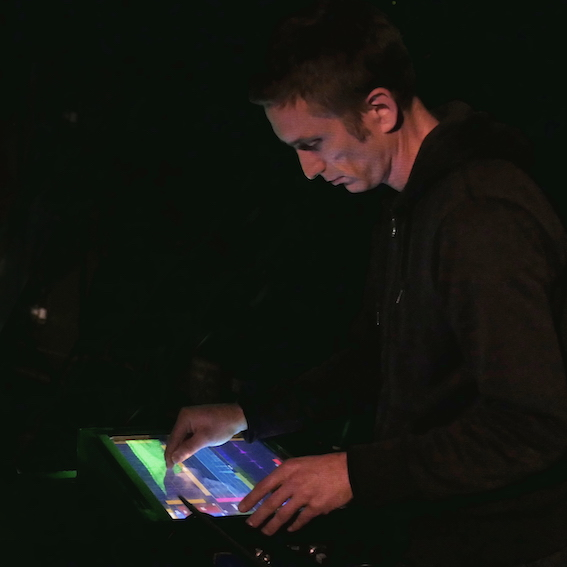
\includegraphics[width=\textwidth]{gfx/05_interfaces/xypre-v1_72dpi.jpg}
	\caption{xypre v1 inauguré durant une performance avec ONE}
	\label{fig:interface:xyprev1_jeu}
\end{figure}

Detecte tout ce qui est en contact (pas seulement les doigts mais aussi les objets) => permet de positionner des éléments de manière stable.

TOTO: insérer photo de la 1ère version (version concert)

\subsubsection{deuxième version}

%-------------------------- Figure : xypre ----------------------------------
\begin{figure}[!htbp]
	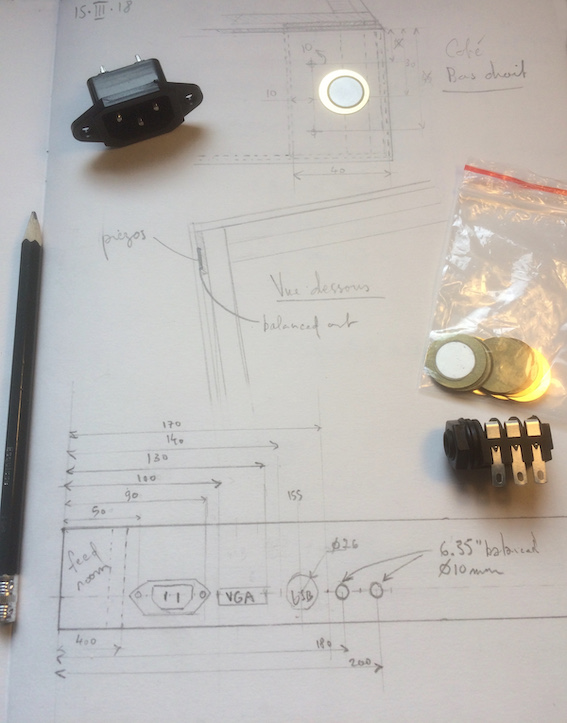
\includegraphics[width=\textwidth]{gfx/05_interfaces/Xypre_plan01_72dpi.jpg}
	\caption{Xypre v2 - plans de conception}
	\label{fig:interface:xypre_plans}
\end{figure}

%-------------------------- Figure : xypre ----------------------------------
\begin{figure}[!htbp]
	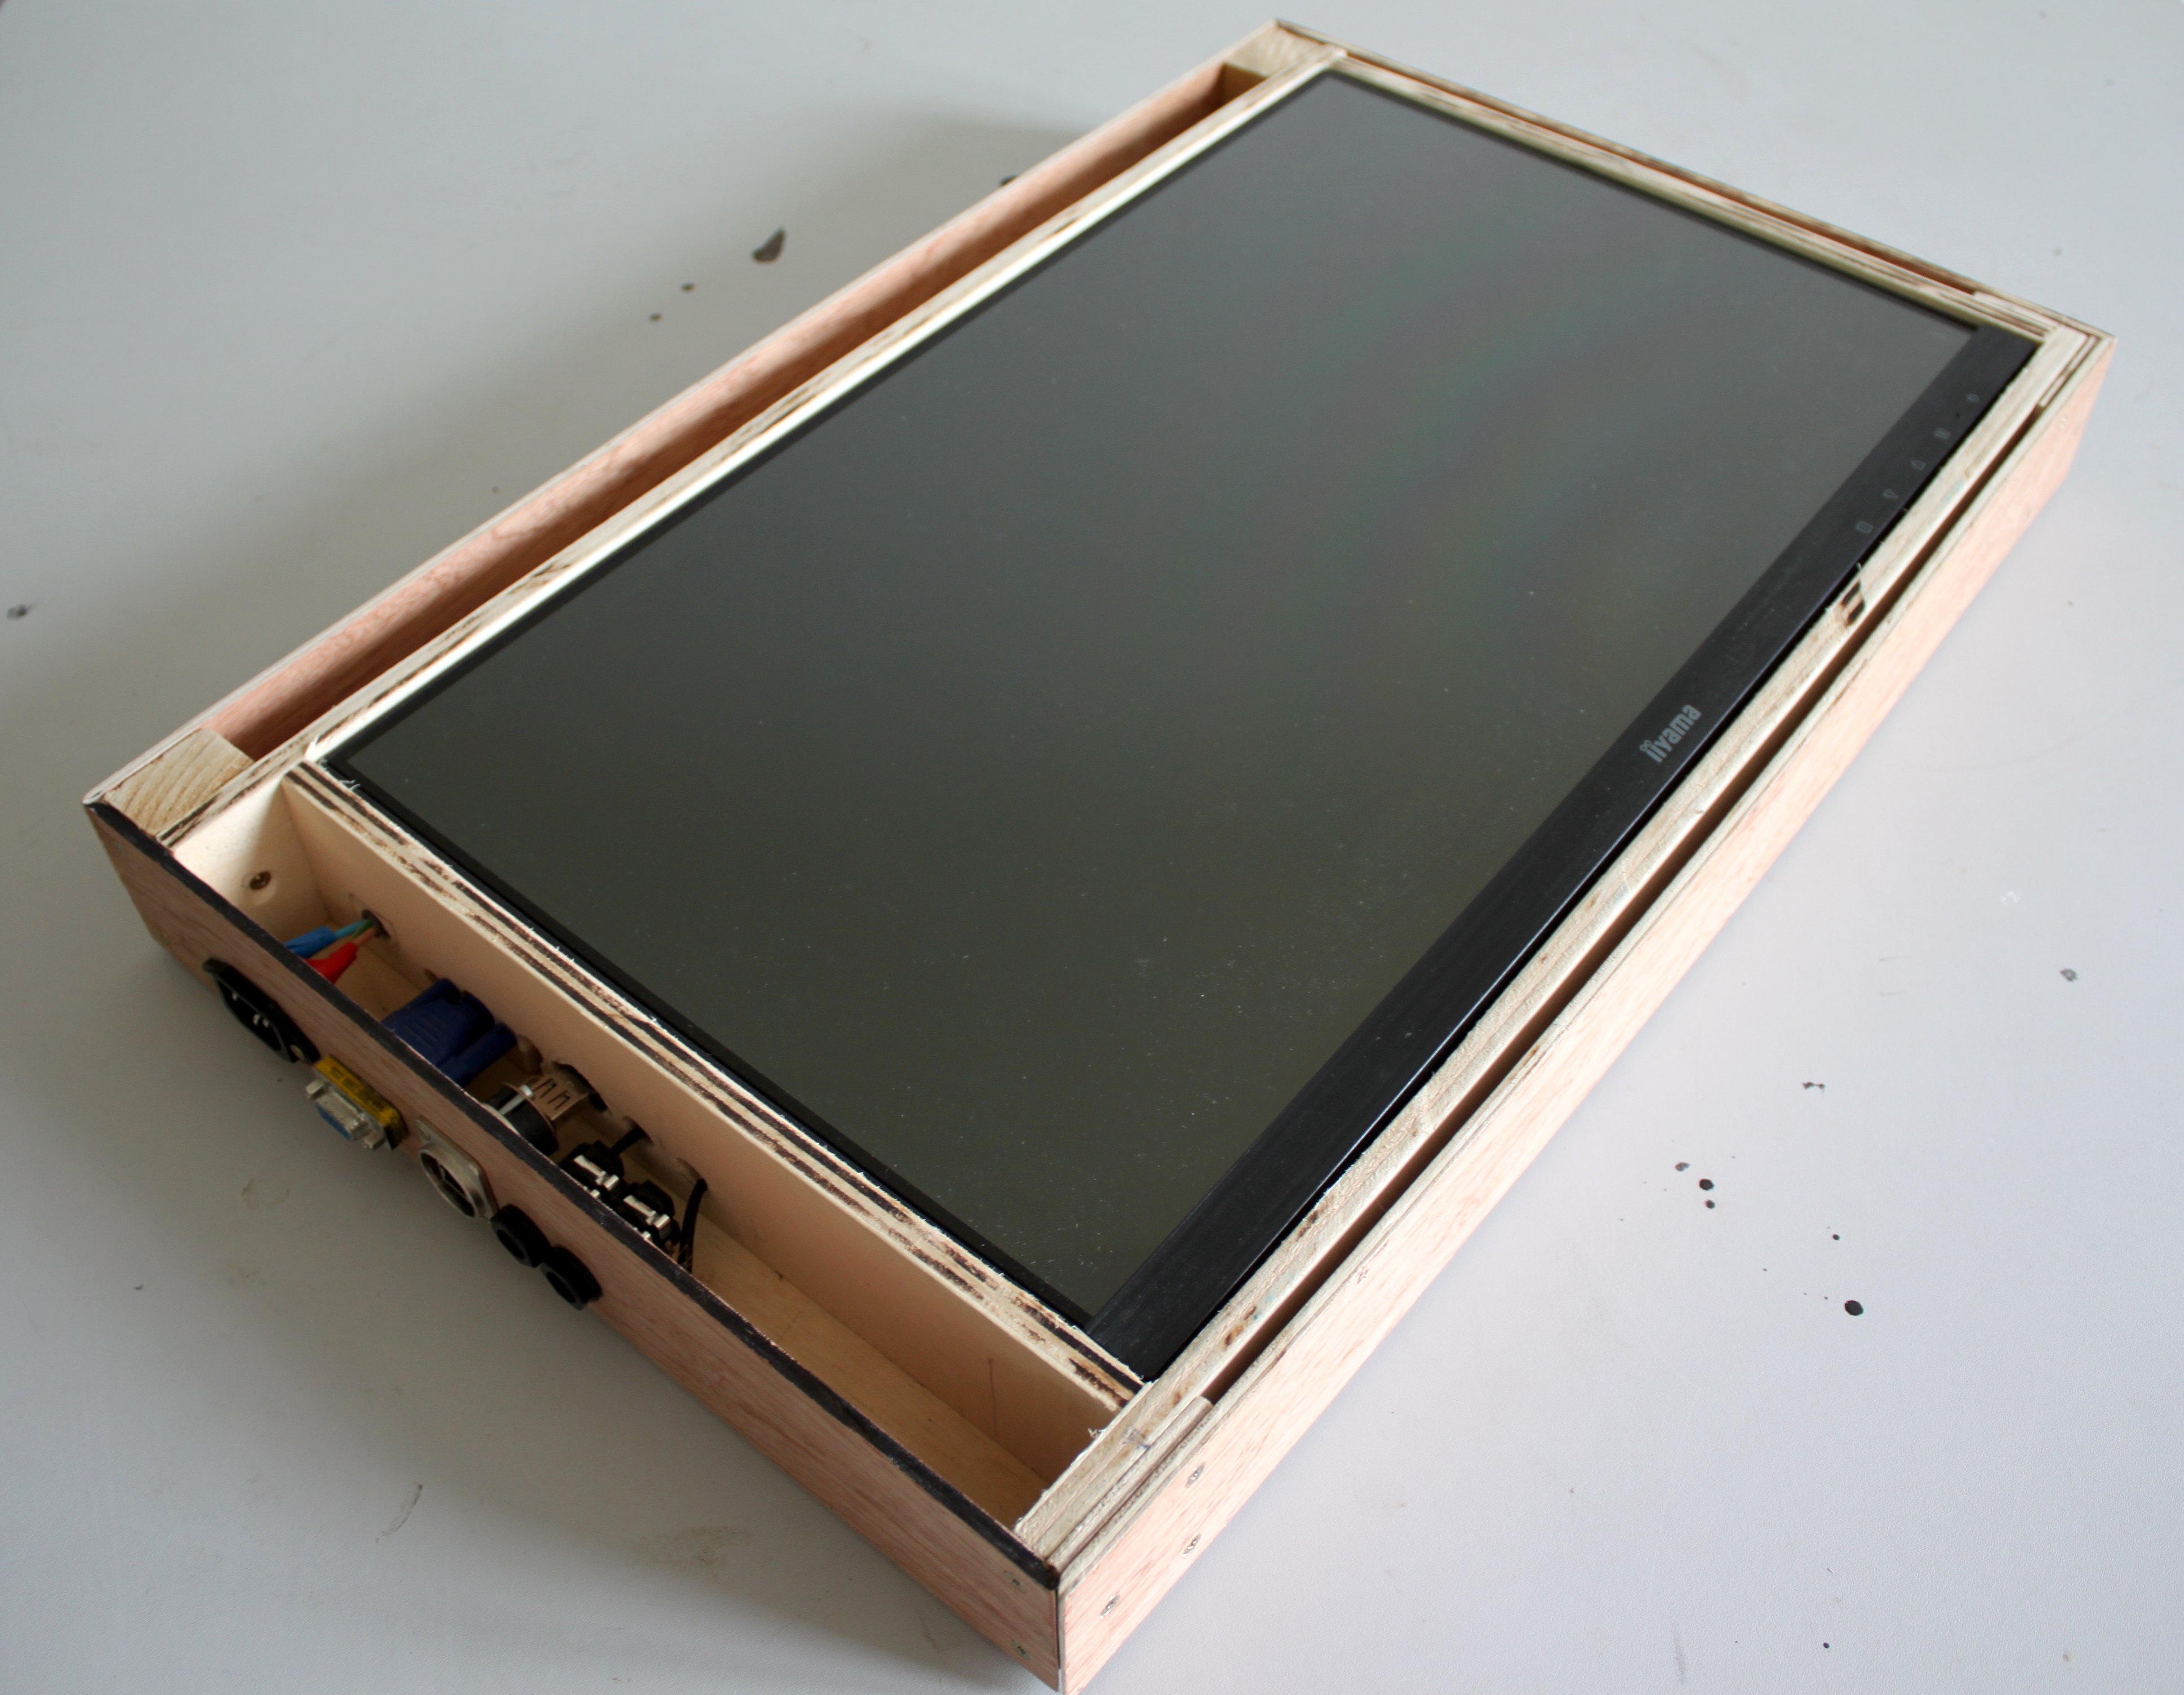
\includegraphics[width=\textwidth]{gfx/05_interfaces/xypre_overview_unplugged.jpg}
	\caption{xypre - vue d'ensemble, débranchée}
	\label{fig:interface:xypre}
\end{figure}

Ecran multitouch capacitif : détecte les doigts uniquement, pas les objets => motivation pour développer des objets positionnables de manière statique dans mp.TUI

Besoin d'un driver payant pour récupérer le TUIO.

Perte de la pression comme paramètre expressif :\\
intégration de capteur de pression (FSR) et de distance (IR)\\
Utilisation d'un Bela pour une latence très faible du son et un instrument autonome (needs raspberry for the display)\\
Possible extension par l'ordinateur.


%%%%%%%%%%%%%%%%%%%%%%%%%%%%%%%%%%%%%%%%%
\section{Conclusion}
\label{sec:interfaces:conclusion}


\section*{extra material}



%%%%%%%%%%%%%%

\iquote{Though there is a huge range of performer decision, history, and knowledge that will determine their exact method of playing (as established by Jorda [12]), the physical design of the DMI impacts this gesture repertoire by presenting certain affordances.} \cite{bin_hands_2017}

